% !TeX root = tcolorbox.tex
% include file of tcolorbox.tex (manual of the LaTeX package tcolorbox)
\clearpage
\section{Macros pour la création des boîtes}%
\tcbset{external/prefix=external/coremacros_}%
\begin{docEnvironment}[doclang/environment content=Contenu de l'environnement]{tcolorbox}{\oarg{options}}
  C'est l'environnement le plus important qui permet de créer une boîte de
  texte mise en évidence de manière colorée avec des angles arrondis et, en
  option, contenant deux parties. L'apparence de cette boîte est contrôlée
  par de nombreuses options. L'exemple le plus simple de code source

\begin{dispListing}
\begin{tcolorbox}
Voici une boîte \textbf{tcolorbox}.
\end{tcolorbox}
\end{dispListing}

crée la boîte de texte compilée suivante
\begin{tcolorbox}
Voici une boîte \textbf{tcolorbox}.
\end{tcolorbox}

Le contenu textuel de la boîte peut être séparé en une partie supérieur «~upper~» et une partie inférieure «~lower~» à l'aide de la commande  \refCom{tcblower}. Les deux parties sont séparées visuellement par une ligne. Par exemple, ce code~:
\begin{dispListing}
\begin{tcolorbox}
Voici une autre boîte \textbf{tcolorbox}.
\tcblower
Ici se trouve la partie inférieure de la boîte.
\end{tcolorbox}
\end{dispListing}
crée la boîte suivante~:

\begin{tcolorbox}
Voici une autre boîte \textbf{tcolorbox}.
\tcblower
Ici se trouve la partie inférieure de la boîte.
\end{tcolorbox}

Les \meta{options} contrôle l'apparence et plusieurs fonctionnalités des boîtes,
consulter la \Vref{sec:optkeys} pour en avoir la liste complète.
Un exemple rapide est donné ici~:

\begin{dispExample}
\begin{tcolorbox}[colback=red!5!white,colframe=red!75!black,title=Mon bel en-tête]
Voici une autre boîte \textbf{tcolorbox}.
\tcblower
Ici se trouve la partie inférieure de la boîte.
\end{tcolorbox}
\end{dispExample}
\end{docEnvironment}

\clearpage
\begin{docCommand}{tcblower}{}
  Cette commande est utilisée à l'intérieur de l'environnement \refEnv{tcolorbox} pour séparer la partie supérieure de la boîte de la partie facultative inférieure de la boîte. Ces deux parties sont traitées comme deux entités fonctionnelles séparées. Si vous voulez seulement tracer une ligne, consultez
  \refCom{tcbline}.
\end{docCommand}

\begin{docCommand}{tcbset}{\marg{options}}
  Définit les options de tous les environnements \refEnv{tcolorbox} suivants, à l'intérieur du groupe \TeX\ actuel.
  Par défaut, elles ne s'appliquent pas aux boîtes imbriquées, voir la \Vref{subsec:everybox}.\par
  Par exemple, les couleurs des boîtes peuvent être définies pour le document complet par~:
\begin{dispListing}
\tcbset{colback=red!5!white,colframe=red!75!black}
\end{dispListing}
\end{docCommand}


\begin{docCommand}{tcbsetforeverylayer}{\marg{options}}
  Définit les options de tous les environnements \refEnv{tcolorbox} suivants, à l'intérieur du groupe \TeX\ actuel.
  Contrairement à \refCom{tcbset}, celles-ci s'appliquent également aux boîtes imbriquées, voir la \Vref{subsec:everybox}.
  Techniquement, ces \meta{options} sont ajoutées aux valeurs par défaut de chaque |tcolorbox|, appliquées par la commande \refKey{/tcb/reset}.\par
  Vous ne devriez pas utiliser cette macro si vous n'êtes pas complètement sûr que vous voulez également appliquer les \meta{options} pour les boîtes dans les boîtes (dans les boîtes, dans les boîtes\ldots).
\begin{dispExample}
\tcbset{colback=green!10!white}
\tcbsetforeverylayer{colframe=red!75!black}

\begin{tcolorbox}[title=Toutes les options pour cette boîte]
  Voici une boîte tcolorbox.\par\medskip
  \begin{tcolorbox}[title=Boîte imbriquée]
    Remarquez que cette boîte imbriquée possède bien un cadre rouge mais pas un arrière-plan vert.
  \end{tcolorbox}
\end{tcolorbox}
\bigskip

\begin{tcolorbox}[reset]
  Les options définies avec |\tcbsetforeverylayer| survivent à un |reset|.
\end{tcolorbox}
\end{dispExample}
\end{docCommand}


\clearpage
\begin{docCommand}{tcbox}{\oarg{options}\marg{contenu de la boîte}}
  Crée une boîte colorée dont la taille est ajustée à la longueur du
  \meta{contenu de la boîte}. En principe, la plupart des \meta{options} d'une
  \refEnv{tcolorbox} peuvent être utilisées pour une |\tcbox| avec quelques restrictions.
  Une boîte |\tcbox| ne peut pas avoir une partie inférieure et ne peut pas être divisée.

\begin{dispExample}
\tcbset{colframe=blue!50!black,colback=white,colupper=red!50!black,
        fonttitle=\bfseries,nobeforeafter,center title}

Texte \tcbox[tcbox raise base]{Bonjour}\hfill
%
\tcbox[left=0mm,right=0mm,top=0mm,bottom=0mm,boxsep=0mm,
  toptitle=0.5mm,bottomtitle=0.5mm,title=Mon tableau]{%
  \arrayrulecolor{blue!50!black}\renewcommand{\arraystretch}{1.2}%
  \begin{tabular}{r|c|l}
  Un   & Deux    & Trois \\\hline\hline
  Homme   & Souris   & Lions \\\hline
  Haut & Milieu & Bas
  \end{tabular}}\hfill
%
\tcbox[colback=blue!85!black,
  left=0mm,right=0mm,top=0mm,bottom=0mm,boxsep=1mm,arc=0mm,boxrule=0.5pt,
  title=Mon dessin]{%
  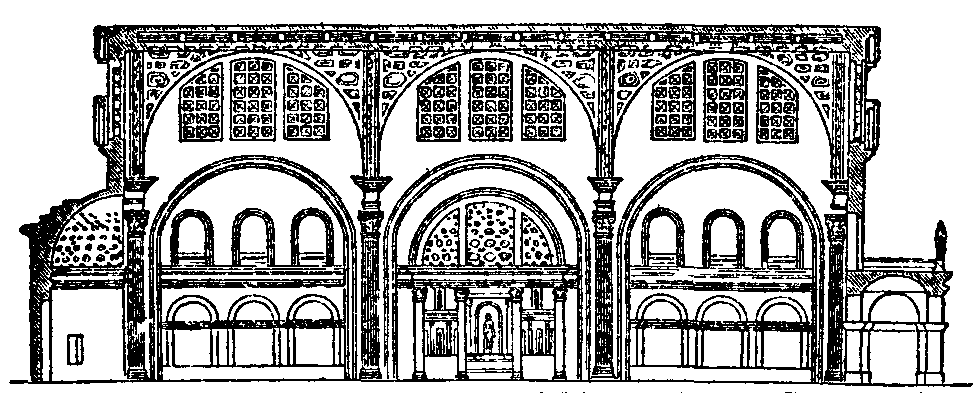
\includegraphics[width=5cm]{Basilica_5.png}}
\end{dispExample}

\begin{dispExample}
% \usepackage{tikz}
\tcbset{colframe=blue!50!black,colback=white,colupper=red!50!black,
        fonttitle=\bfseries,center title}

% Boîte de longueur fixée
\begin{tcolorbox}Bonjour\\le monde~!\end{tcolorbox}

% Boîte de largeur « ajustée » (comme hbox ou makebox)
\tcbox{Bonjour\\le monde~!}

% Boîte de largeur « ajustée » (utilisant un noeud \tikzname)
\tcbox[tikznode]{Bonjour\\le monde~!}
\end{dispExample}

\end{docCommand}

\clearpage
\begin{marker}
Consultez la section \ref{subsec:xparse_tcolorbox} à la page \pageref{subsec:xparse_tcolorbox}
et la section \ref{subsec:xparse_tcbox} à la page \pageref{subsec:xparse_tcboxfit} pour apprendre d'autres méthodes plus élaborées pour créer de nouveaux environnements et nouvelles commandes.
\end{marker}

\begin{docCommand}{newtcolorbox}{\oarg{options d'initialisation}\marg{nom}\oarg{nombre}\oarg{défaut}\marg{options}}
  Crée un nouvel environnement appelé \meta{nom} basé sur \refEnv{tcolorbox}.
  |\newtcolorbox| fonctionne tout simplement comme |\newenvironment|. Cela signifie que 
  le nouvel environnement \meta{nom} peut prendre en option \meta{nombre} arguments, où
  \meta{défaut} (qui est également optionnel) est la valeur par défaut du premier argument 
  de l'environnement qui devient alors optionnel. Les \meta{options} sont transmises 
  au |tcolorbox| sous-jacent.
  Notez que \refKey{/tcb/savedelimiter} prend automatiquement comme valeur le \meta{nom} fourni.
  Les \meta{options d'initialisation} permettent le paramétrage d'une numérotation automatique,
  consultez la section \ref{sec:initkeys} à la page \pageref{sec:initkeys}.
\begin{dispExample*}{sbs,lefthand ratio=0.6}
\newtcolorbox{maboite}{colback=red!5!white,
  colframe=red!75!black}

\begin{maboite}
Voici ma boîte personnelle.
\end{maboite}
\end{dispExample*}

\begin{dispExample*}{sbs,lefthand ratio=0.6}
\newtcolorbox{maboite}[1]{colback=red!5!white,
  colframe=red!75!black,fonttitle=\bfseries,
  title={#1}}

\begin{maboite}{Salut à tous}
Voici ma boîte personnelle avec un titre
obligatoire.
\end{maboite}
\end{dispExample*}

\begin{dispExample*}{sbs,lefthand ratio=0.6}
\newtcolorbox{maboite}[2][]{colback=red!5!white,
  colframe=red!75!black,fonttitle=\bfseries,
  colbacktitle=red!85!black,enhanced,
attach boxed title to top center={yshift=-2mm},
  title={#2},#1}

\begin{maboite}[colback=yellow]{Salut à tous}
Voici ma boîte personnelle avec un titre
obligatoire et des options.
\end{maboite}
\end{dispExample*}

\inputpreamblelisting{A}

\begin{dispExample*}{sbs,lefthand ratio=0.6}
\begin{pabox}[colback=yellow]{Salut à tous}
Voici ma boîte personnelle avec un titre
obligatoire numéroté et des options.
\end{pabox}
\end{dispExample*}
\end{docCommand}


\begin{docCommand}{renewtcolorbox}{\oarg{options d'initialisation}\marg{nom}\oarg{nombre}\oarg{défaut}\marg{options}}
  Fonctionne comme \refCom{newtcolorbox} mais basé sur |\renewenvironment| au lieu de |\newenvironment|.
  Un environnement existant est redéfini.
\end{docCommand}


\clearpage
\begin{docCommand}{newtcbox}{\oarg{options d'initialisation}\brackets{\texttt{\textbackslash}\meta{nom}}\oarg{nombre}\oarg{défaut}\marg{options}}
  Crée une nouvelle macro appelée \texttt{\textbackslash}\meta{nom} basé sur \refCom{tcbox}.
  |\newtcbox| fonctionne tout simplement comme |\newcommand|.
  La nouvelle macro \texttt{\textbackslash}\meta{nom} peut prendre  \meta{nombre}$+1$ arguments, où
  \meta{défaut} est la valeur par défaut du premier
  argument de l'environnement qui devient optionnel.
  Les \meta{options} sont transmises au |tcbox| sous-jacent.
  Les \meta{options d'initialisation} permettent le paramétrage de la numérotation automatique, consultez la section~\ref{sec:initkeys} à la page~\pageref{sec:initkeys}.
\begin{dispExample*}{sbs,lefthand ratio=0.6}
\newtcbox{\mybox}{colback=red!5!white,
  colframe=red!75!black}

\mybox{Voici ma boîte personnelle.}
\end{dispExample*}

\begin{dispExample*}{sbs,lefthand ratio=0.6}
\newtcbox{\mybox}[1]{colback=red!5!white,
  colframe=red!75!black,fonttitle=\bfseries,
  title={#1}}

\mybox{Salut à tous}{Voici ma boîte personnelle.}
\end{dispExample*}

\begin{dispExample*}{sbs,lefthand ratio=0.6}
\newtcbox{\mybox}[2][]{colback=red!5!white,
  colframe=red!75!black,fonttitle=\bfseries,
  title={#2},#1}

\mybox[colback=yellow]{Salut à tous}%
  {Voici ma boîte personnelle.}
\end{dispExample*}

\inputpreamblelisting{B}

\begin{dispExample*}{sbs,lefthand ratio=0.6}
\pbbox[colback=yellow]{Salut à tous}%
  {Voici ma boîte personnelle.}
\end{dispExample*}

\begin{dispExample}
\newtcbox{\mybox}[1][red]{on line,
  arc=0pt,outer arc=0pt,colback=#1!10!white,colframe=#1!50!black,
  boxsep=0pt,left=1pt,right=1pt,top=2pt,bottom=2pt,
  boxrule=0pt,bottomrule=1pt,toprule=1pt}
\newtcbox{\xmybox}[1][red]{on line,
  arc=7pt,colback=#1!10!white,colframe=#1!50!black,
  before upper={\rule[-3pt]{0pt}{10pt}},boxrule=1pt,
  boxsep=0pt,left=6pt,right=6pt,top=2pt,bottom=2pt}

The \mybox[green]{quick} brown \mybox{fox} \mybox[blue]{jumps} over the
\mybox[green]{lazy} \mybox{dog}.\par
The \xmybox[green]{quick} brown \xmybox{fox} \xmybox[blue]{jumps} over the
\xmybox[green]{lazy} \xmybox{dog}.
\end{dispExample}

\end{docCommand}

%\enlargethispage*{1cm}

\clearpage
\begin{docCommand}{renewtcbox}{\oarg{options d'initialisation}\brackets{\texttt{\textbackslash}\meta{nom}}\oarg{nombre}\oarg{défaut}\marg{options}}
  Fonctionne comme \refCom{newtcbox} mais basé sur |\renewcommand| au lieu de |\newcommand|.
  Une macro existante est redéfinie.
\end{docCommand}



\begin{docCommand}[doc new=2014-10-20]{tcolorboxenvironment}{\marg{nom}\marg{options}}
  L'environnement existant appelé \meta{nom} est redéfini afin d'être mis en boîte dans une
  |tcolorbox| en utilisant les options \meta{options}.
\begin{dispExample*}{sbs,lefthand ratio=0.6}
% tcbuselibrary{skins}
\newenvironment{maliste}{%
  \begin{itemize}}{\end{itemize}}

\tcolorboxenvironment{maliste}{blanker,
  before skip=6pt,after skip=6pt,
  borderline west={3mm}{0pt}{red}}

Du texte.
\begin{maliste}
\item Alpha
\item Beta
\item Gamma
\end{maliste}
Encore du texte.
\end{dispExample*}

\medskip
Consultez d'autres exemples à la section \ref{subsec:theorems_other} à la page \pageref{subsec:theorems_other}.
\end{docCommand}
